\documentclass[a4paper, 10pt,onecolumn]{scrartcl}
\usepackage[ngerman]{babel}
\usepackage[T1]{fontenc}
\usepackage[utf8]{inputenc}
\usepackage{multirow}
\usepackage{natbib}
\usepackage{graphicx}
\usepackage{amsmath, amssymb}
\usepackage{graphicx}
\usepackage{grffile} %einfacheres einbinden von Dateipfaden
\usepackage{xpatch} %more space between title and subtitle
\usepackage{mathtools}

\newlength{\myspace}
\setlength{\myspace}{2em}

\makeatletter
\xpatchcmd{\@maketitle}{\vskip.5em}{\vskip\myspace}{}{}
\makeatother



\title{Computational Physics 1: Übung 4: Downhill-Simplex-Verfahren} 
\author{Jakob Hollweck} %auch nach \begindocument möglich
\setlength{\parindent}{0pt}
\date{Abgabe 01.12.17}

\begin{document}
\maketitle


\section*{\centerline {Untersuchung des Konvergenzverhaltens}} 

\begin{figure}[ht!]
	\centering
	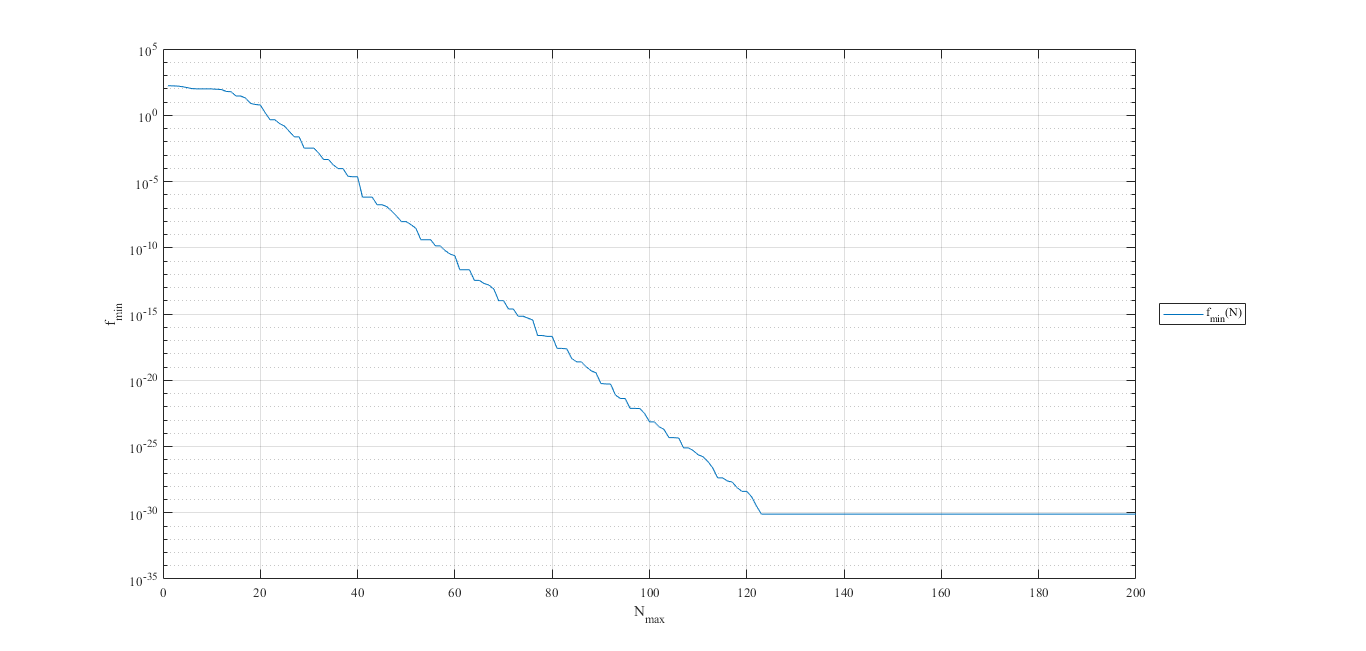
\includegraphics[scale=0.4]{DS.png}
	\caption{$f_{min}$ über $N_{max}$} 
	\label{Abbildung1}
\end{figure}

Das erarbeitete Skript zum Berechnen der Minima einer zweidimensionalen Funktion liefert für den Fall einer maximalen Genauigkeit von $p$=0 im Intervall [-1,-1] den durch Abbildung \ref{Abbildung1} gegebenen Graphen.
Es ist zu erkennen, dass $f_{min}$ für größer werdende $N_{max}$ exponentiell abnimmt (Logarithmische Skala), das Verfahren konvergiert also exponentiell bezüglich der Genauigkeit.
Bei etwas mehr als 120 Schritten stagniert $f_{min}$ bei $10^{-30}$ für alle größeren $N_{max}$. Der Grund dafür könnte sein, dass das verwendete Zahlenformat hier an seine Genauigkeitsgrenzen stößt. Dagegen spricht, dass das von Matlab verwendete "`Real"'-Zahlenformat dies erst bei ca. $10^{-38}$ tun sollte. Die leichte Stufigkeit der Kurve könnte von den vielen verschiedenen Möglichkeiten herrühren, einen Simplex zu bilden, die teilweise untereinander nicht alle gleich effizient sind.

\section*{\centerline {Zusammenhang zwischen Minimum und Startwert}} 
Der Zusammenhang zwischen gewählten Startkoordinaten und gefundenem Minimum ist im Allgemeinen, dass nur ein lokales Minimum der gegebenen Funktion gefunden werden kann. Die Funktionsweise des Verfahrens ist, dass durch verschiedene Ausführungen von Spiegelung, Kontraktion und Expansion immer der Punkt mit dem höchsten Funktionswert durch einen Punkt mit niedrigerem Funktionswert ersetzt wird.  Die erfolgreiche Benutzung dieser setzt also ein Grundverständnis des Problems und eine ungefähre Kenntnis der Extrema voraus.

\end{document}